\documentclass[11pt]{article}
\usepackage[margin=1in]{geometry}
\usepackage{amsmath,amssymb,bm}
\usepackage{graphicx}\usepackage{booktabs}\usepackage{caption}
\usepackage[table]{xcolor}\usepackage{hyperref}
\hypersetup{colorlinks=true,linkcolor=blue!50!black}
\graphicspath{{figs/}}\captionsetup{font=small}
\newcommand{\Rd}{\mathbb{R}}
\title{\textbf{Element-wise affine memory modulation in a recurrent vision transformer:\\
attention dynamics, and a perceived-but-discarded validity cue}}
\author{Recurrent Vision Transformer Project --- single-variant analysis (\texttt{affine\_ew})}
\date{Checkpoint: conv front-end $+$ element-wise affine self-attention $+$ JEPA, iteration 4{,}199 ($\approx0.83$ correct)}
\begin{document}\maketitle
\begin{abstract}\noindent
We analyse a recurrent vision transformer in which the recurrent memory modulates the visual features by
an \emph{element-wise affine} transform (a learned per-feature scale and shift, no identity term) before a
standard self-attention over the four stimulus patches---a diagonal alternative to cross-attention and to
matrix-valued FiLM. On the cued change-detection task the agent reaches $\approx0.83$ correct. Its
attention follows a transient-orient / re-acquire / bottom-up-lock schedule: it focuses the cued patch at
the cue frame, releases it during the blank, re-acquires it as the stimuli appear, and locks onto an
orientation change when it occurs. Critically, the change-lock is \emph{bottom-up}: it captures both
validly and invalidly cued changes on the change frame. We then test, properly, whether cue validity
(ring proportion) and cue value (colour) modulate attention and behaviour. Attention is invariant to both.
Decoding the recurrent state explains why for validity: proportion is decoded almost perfectly at the cue
frame ($0.99$) but is \emph{discarded} within two frames (chance by the stimulus onset), whereas cue
position and value are retained throughout. Consequently the displayed validity neither shapes attention
nor scales the behavioural cueing benefit; the benefit that exists ($\sim0.2$ higher detection for validly
cued changes at threshold magnitudes) is carried by the maintained spatial cue, not the validity ring.
\end{abstract}

\section{Model and task}
The task is the $T{=}7$-frame cued orientation-change-detection task (blank, cue, blank, four Gabors at
$t{=}3$--$6$, a single orientation step at $t{=}5$ on half of trials), with a coloured cue marking one of
four quadrants $[S1,\text{TR},\text{BL},S4]$; colour signals value (red$=5$, green$=3$, blue$=1$) and ring
completeness signals validity (proportion $p\in\{.25,.5,.75,1.0\}$). The agent emits \texttt{wait}/
\texttt{declare-change} each frame. The front-end is a shared SE-ResNet encoding each $25\times25$ patch to
$\hat o_i\in\Rd^{128}$; tokens are $\bm x_i=[\hat o_i\Vert\bm\rho_i\Vert\bm\tau]\in\Rd^{140}$.

\paragraph{Element-wise affine self-attention.} Let $H^{(t-1)}\in\Rd^{4\times128}$ be the per-patch xLSTM
cell. The block modulates each token by a memory-derived per-feature scale $\bm\gamma$ and shift
$\bm\beta$ and then self-attends over the four patches:
\begin{align}
\bm b=\tanh(H^{(t-1)}W_b),\quad
\bm\gamma=\bm b\,W_\gamma\in\Rd^{4\times140},\quad \bm\beta=\bm b\,W_\beta\in\Rd^{4\times140},\\
X' = \bm\gamma\odot X + \bm\beta\quad(\text{element-wise; no $1{+}$ identity, } \bm\gamma\!\to\!1,\bm\beta\!\to\!0\text{ at init}),\\
Q,K,V = X'W_q,\,X'W_k,\,X'W_v,\qquad
\boxed{\,A^{(t)}=\mathrm{softmax}\!\Big(\tfrac{QK^\top}{\sqrt{140}}\Big)\in\Rd^{4\times4}\,},\qquad Z=X+A^{(t)}V .
\end{align}
Unlike the cross-attention variant, the keys are the four (modulated) image patches only---there is no
separate memory-key column; the memory acts entirely through $(\bm\gamma,\bm\beta)$. Hence $A^{(t)}_{ij}$
is the attention from query patch $i$ to image patch $j$, each row summing to $1$ (uniform $=0.25$). $Z$
drives the per-patch xLSTM; the flattened cell feeds a 3-ELU actor and a QR-DQN critic; training is
reward-only with an auxiliary V-JEPA temporal self-distillation loss. We report $A^{(t)}$ averaged over
$96$ trials per condition (raw softmax weights, no further normalisation), always exercising the
validity manipulation \emph{both ways} (change at the cued and at an uncued patch). Detection rates are
$P(\text{press}\ge t_{\text{chg}})$ over $150$ episodes; decoding is 4-fold CV logistic regression on the
flattened cell.

\section{Results}
\subsection{Attention schedule: orient, release, re-acquire, lock}
The agent is correct on $\approx0.83$ of natural trials. Its attention to the cued patch
(Fig.~\ref{fig:tc}, left) rises to $0.73$ at the cue frame, falls to chance during the following blank
($0.22$ at $t{=}2$), then \emph{re-acquires} the cued location as the Gabors appear ($0.44\to0.80$ over
$t{=}3,4$), and saturates at $1.0$ when a (cued) change occurs. The full $4\times4$ maps across all six
cue$\times$change conditions are in Fig.~\ref{fig:maps}.

\begin{figure}[h]\centering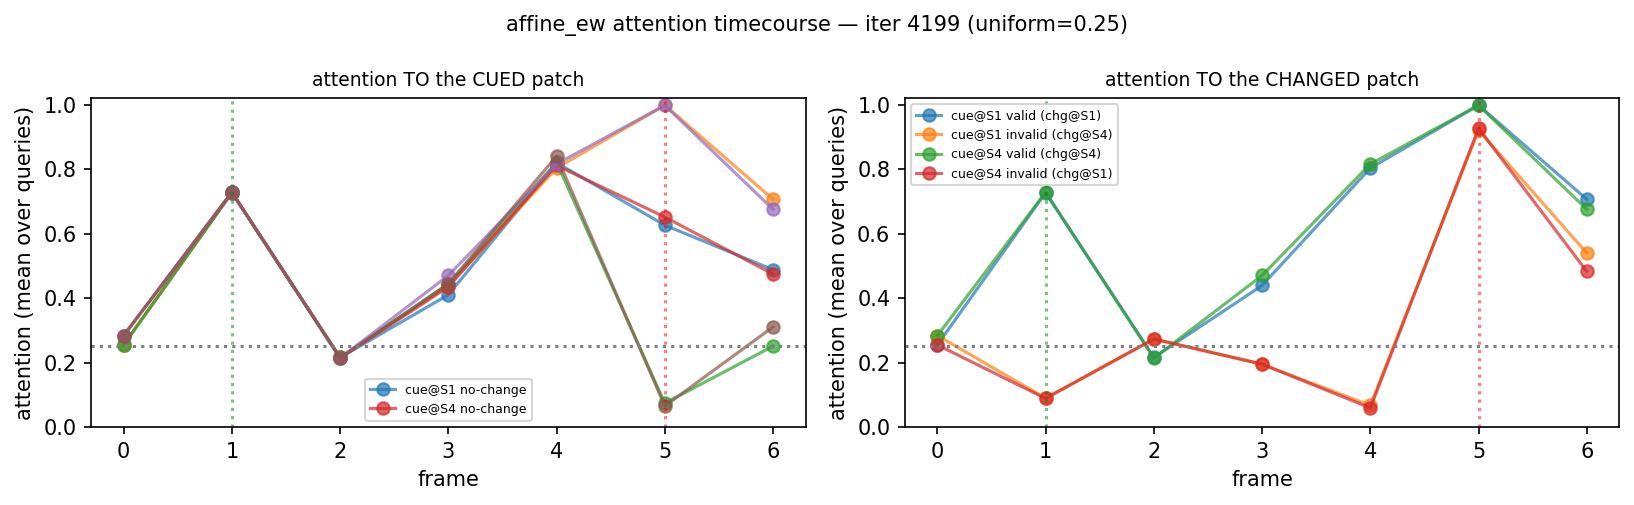
\includegraphics[width=\textwidth]{dda_timecourse.png}
\caption{\textbf{Attention timecourse} (mean over queries; uniform $=0.25$). Left: attention to the cued
patch---transient orient at the cue ($t{=}1$), release at the blank ($t{=}2$), re-acquisition over the
Gabor frames. Right: attention to the changed patch---the lock at $t{=}5$ for both valid and invalid
changes.}\label{fig:tc}\end{figure}

\subsection{The change-lock is bottom-up (valid and invalid)}
When a change occurs, attention locks onto the changed patch \emph{on the change frame} regardless of
whether it was cued: attention to the changed patch at $t{=}5$ is $1.00$ (valid) and $0.92$ (invalid),
decaying by $t{=}6$ ($0.71$ / $0.54$). The element-wise affine block thus implements a bottom-up
salience grab---any large orientation step pulls attention---in contrast to the cross-attention variant,
whose memory change-lock for invalid changes is delayed by a frame. This predicts a smaller behavioural
cueing benefit, since invalid changes are still attended (Sec.~3.4).

\begin{figure}[h]\centering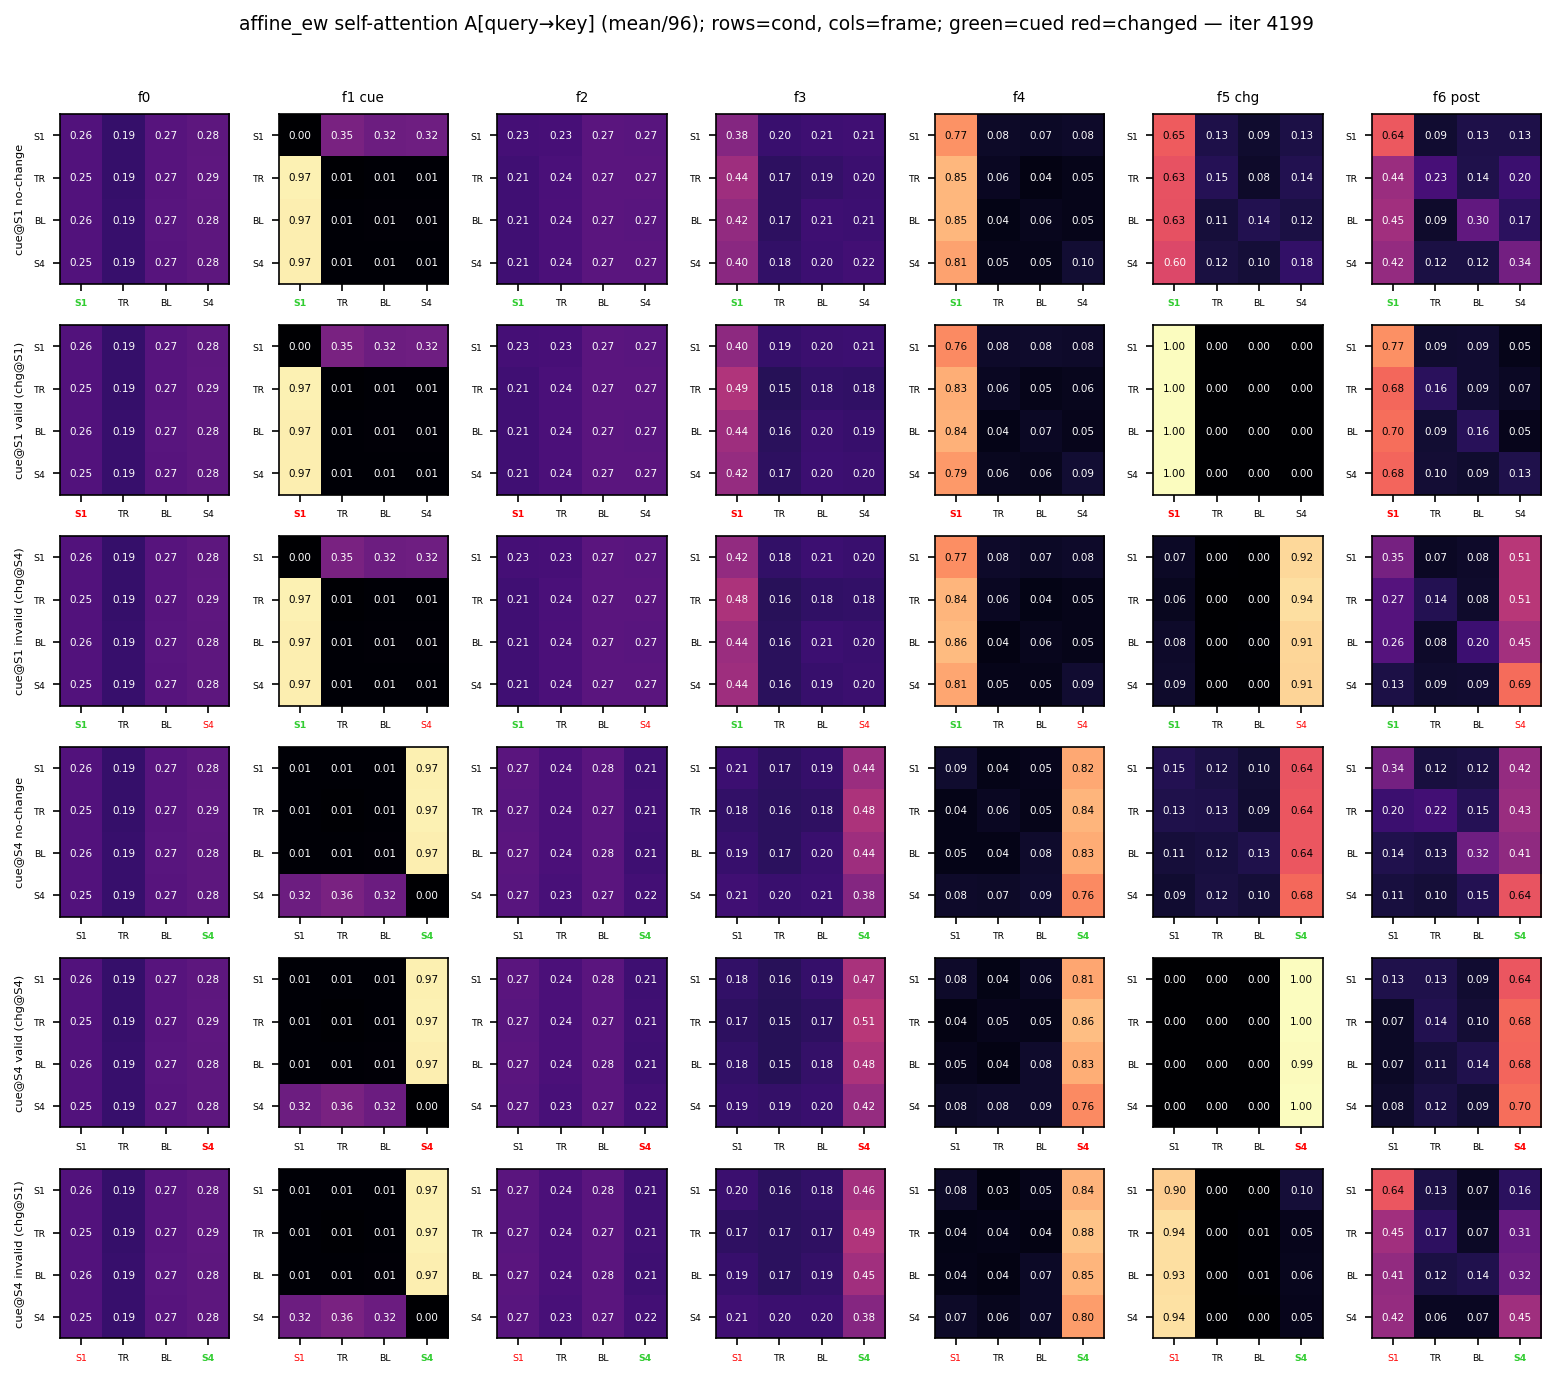
\includegraphics[width=\textwidth]{dda_maps.png}
\caption{\textbf{Raw self-attention maps} $A[\text{query}\to\text{key}]$, mean over $96$ trials. Rows:
six cue$\times$change conditions; columns: frames $0$--$6$; within a tile, rows are query patches and
columns are key (image) patches $[S1,\text{TR},\text{BL},S4]$ (green $=$ cued, red $=$ changed).}
\label{fig:maps}\end{figure}

\subsection{Cue validity (proportion) does not modulate attention}
Exercising validity properly---valid \emph{and} invalid changes at every proportion, both cue
positions---attention is flat across $p\in\{.25,\dots,1.0\}$ (Fig.~\ref{fig:propattn}): the cue-frame
focus stays at $\approx0.72$, gabor-phase monitoring of the cued patch at $\approx0.62$, and the
change-lock (valid and invalid) is unchanged. The model does not broaden its monitoring when the cue is
unreliable.

\begin{figure}[h]\centering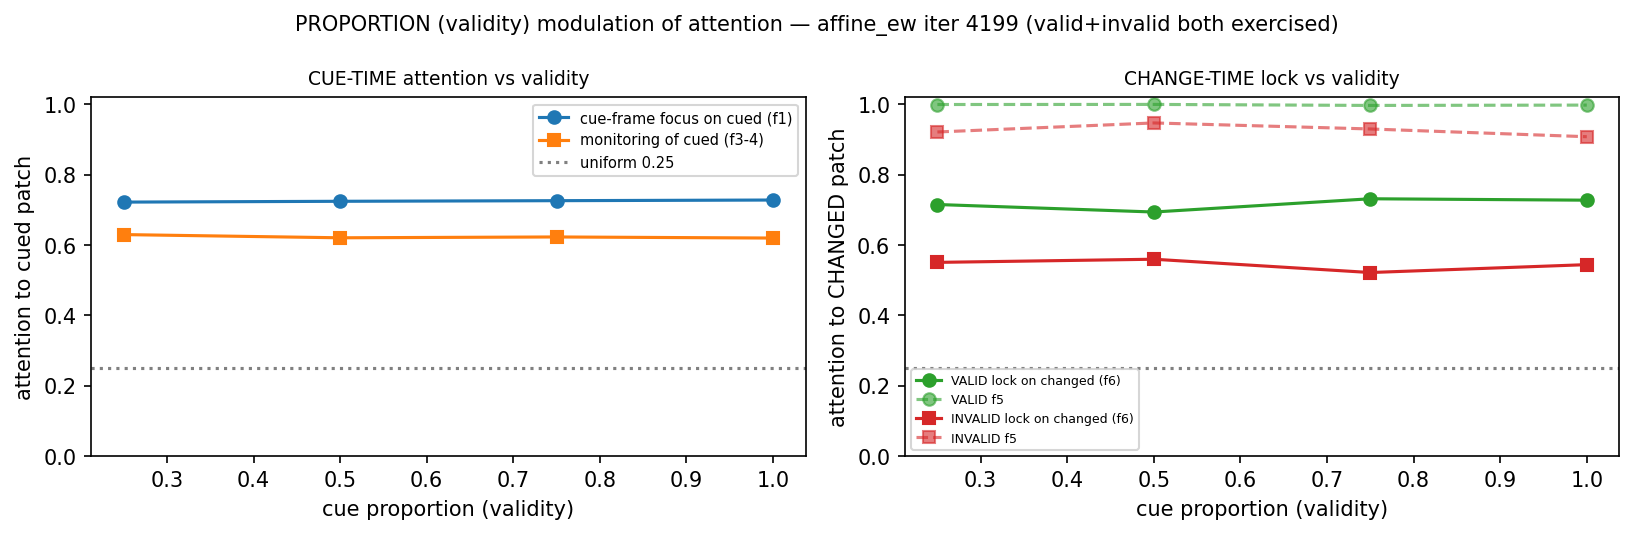
\includegraphics[width=0.92\textwidth]{dda_prop_attn_metrics.png}
\caption{\textbf{Validity sweep of attention.} Cue-time focus / monitoring (left) and change-time lock
for valid and invalid changes (right) vs.\ displayed proportion. All flat: attention is validity-invariant.
Raw maps per proportion in \texttt{dda\_prop\_maps\_valid/invalid}.}\label{fig:propattn}\end{figure}

\subsection{Why: validity is perceived at the cue then discarded}
Decoding the recurrent cell resolves the invariance (Fig.~\ref{fig:dec}). Cue position and cue value are
decoded near-perfectly from the cue frame onward and \emph{maintained} for the rest of the trial.
Proportion (validity) is also read at the cue frame---decodable at $0.99$ at $t{=}1$ and $0.96$ at
$t{=}2$---but is then \emph{discarded}: decoding falls to chance ($0.22$) by the Gabor onset ($t{=}3$)
and stays there through the change. The validity ring is perceived but not retained; by the time a change
must be judged, the model no longer represents how reliable the cue was. This is the mechanistic reason
attention and the decision cannot scale with validity.

\begin{figure}[h]\centering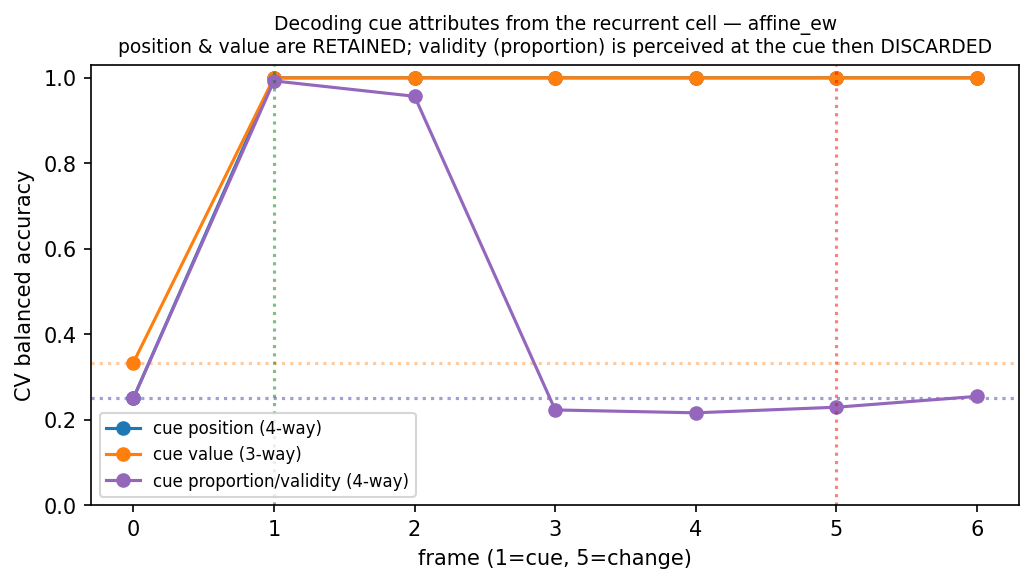
\includegraphics[width=0.72\textwidth]{dda_decoding.png}
\caption{\textbf{Decoding cue attributes from the recurrent cell.} Position and value are retained
(flat at ceiling); proportion (purple) spikes to $0.99$ at the cue frame and collapses to chance by the
stimulus onset---perceived, then discarded.}\label{fig:dec}\end{figure}

\subsection{Behaviour: a spatial cueing benefit that does not scale with validity}
There is nonetheless a genuine cueing benefit: validly cued changes are detected at lower magnitude than
invalidly cued ones (Fig.~\ref{fig:psy}), e.g.\ at proportion $1.0$ and $|\Delta\theta|=16^\circ$,
$P(\text{detect})=0.43$ (valid) vs.\ $0.21$ (invalid). But the benefit is carried by the maintained
\emph{spatial} cue, not the validity magnitude: the valid$-$invalid gap at threshold magnitudes
($12$--$20^\circ$) is $\approx0.21,0.23,0.19,0.25$ across proportions $.25,.5,.75,1.0$---essentially
constant (Fig.~\ref{fig:gap}), exactly as expected if proportion is unavailable at decision time.

\begin{figure}[h]\centering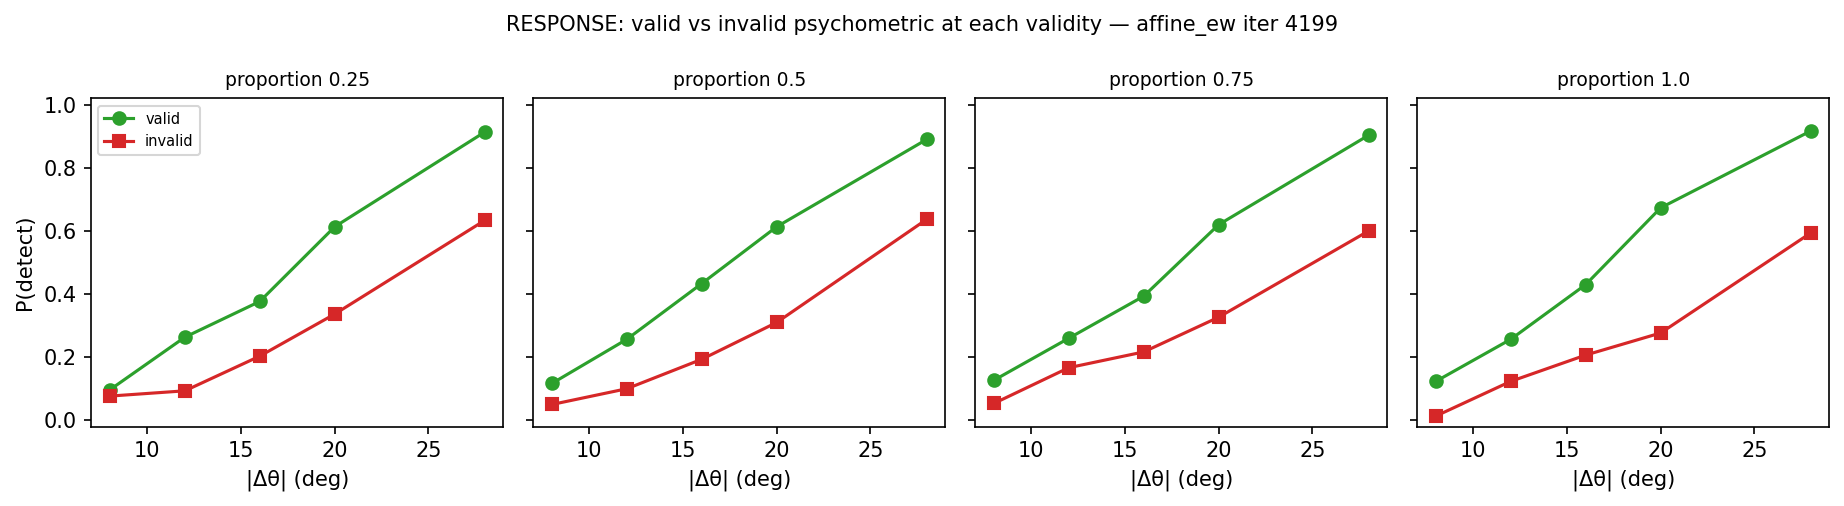
\includegraphics[width=\textwidth]{dda_resp_psych_by_prop.png}
\caption{\textbf{Valid vs.\ invalid psychometric at each validity.} A consistent valid$>$invalid benefit
at every proportion; the curves do not separate more at higher displayed validity.}\label{fig:psy}\end{figure}
\begin{figure}[h]\centering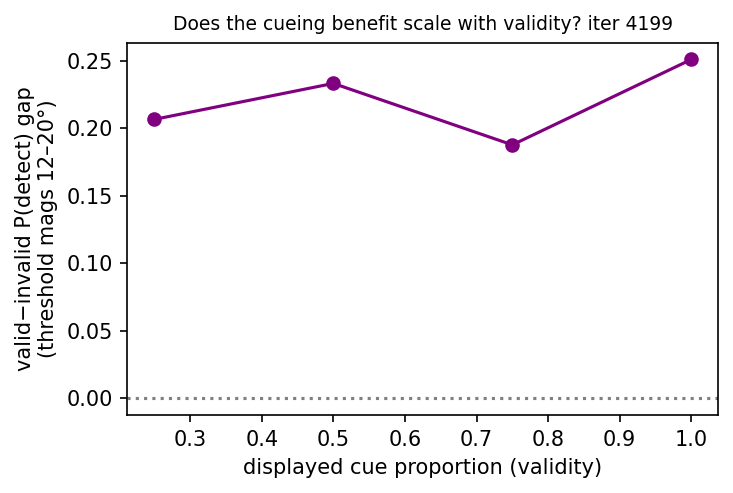
\includegraphics[width=0.5\textwidth]{dda_resp_gap_vs_prop.png}
\caption{\textbf{Cueing benefit vs.\ displayed validity.} The valid$-$invalid detection gap (threshold
magnitudes) is flat across proportion---the benefit is spatial, not validity-graded.}\label{fig:gap}\end{figure}

\subsection{Cue value (colour)}
Unlike validity, value \emph{is} retained (decoded at ceiling from the cue frame through the trial;
Fig.~\ref{fig:dec}), so it is available to the decision---and it has a mild effect there
(Fig.~\ref{fig:val}). High-value (red) changes are detected slightly better than low-value ones at
threshold and supra-threshold magnitudes ($|\Delta\theta|=20^\circ$: red $0.59$, blue $0.54$, green
$0.50$; $28^\circ$: red $0.90>$ green $0.85>$ blue $0.81$), an ordering consistent with the agent being
modestly more eager to report a valuable change. The attention itself is not cleanly value-graded: the
cue-frame focus varies with \emph{colour} ($0.89$ blue, $0.74$ green, $0.73$ red) but \emph{not}
monotonically with value, indicating a low-level colour-appearance effect on the front-end rather than a
value-driven attentional gain; the change-lock is essentially value-invariant. Thus value enters the
\emph{decision} (via the retained value code), not the attention map---the same deployment-vs-use
dissociation seen for the spatial cue, and the opposite of validity, which is not retained at all. The
value effect is small, as expected for this early checkpoint.

\begin{figure}[h]\centering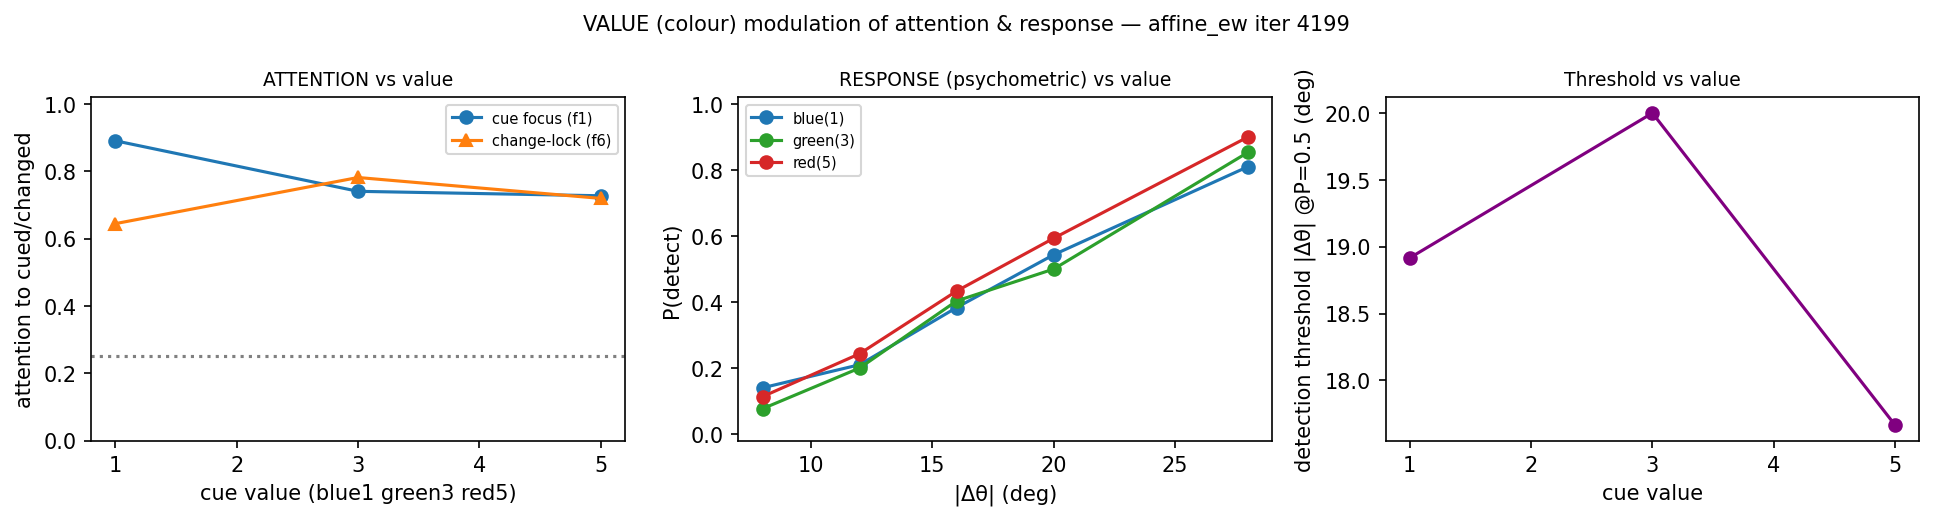
\includegraphics[width=\textwidth]{dda_value.png}
\caption{\textbf{Value (colour) modulation.} Left: attention vs.\ value (cue focus varies by colour but
not monotonically with value). Middle: detection psychometric per colour---red (value $5$) is detected
best. Right: detection threshold vs.\ value. Maps per colour in \texttt{dda\_value\_maps}.}
\label{fig:val}\end{figure}

\section{Discussion}
The element-wise affine variant learns a legible attentional schedule---transiently orient to the cue,
release, re-acquire the cued location as evidence arrives, and lock onto a change---and detects changes
through a \emph{bottom-up} lock that fires for cued and uncued changes alike. The most informative result
is a dissociation in what the recurrence keeps: the spatial cue and its value are maintained, but the
validity ring is perceived and then discarded within two frames. This single fact accounts for the
otherwise puzzling invariance of both attention and the cueing benefit to displayed validity, and it is a
concrete, falsifiable claim about the agent's internal economy of memory. That the agent still shows a
spatial cueing benefit while ignoring validity magnitude mirrors a known dissociation in covert attention
between \emph{where} attention is allocated and \emph{how} cue reliability is used. Whether longer training
(this checkpoint is early, $\approx0.83$) leads the agent to retain validity, and whether the retained
value signal modulates the decision (Sec.~3.6), are the natural next questions.

\end{document}
